\section{Base teórica}
\subsection*{Neurobiologia básica}
\begin{frame}
	\begin{columns}[t]
		\column{5cm}
			\begin{figure}[tb]
				\centering
				\caption{Neurônio}
				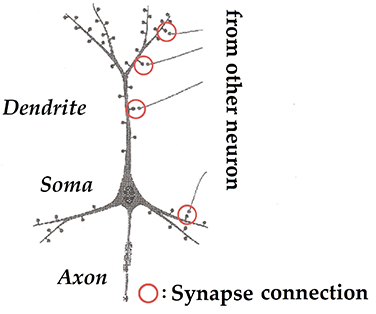
\includegraphics[width=0.55\linewidth]{figs/neuronio}
				\label{fig:neuronio}
				%		\fonte{Adaptado de \cite{lopez-ruiz_simulation_2016}}
				%TODO: trocar figura
			\end{figure}
		\column{5cm}
			\begin{itemize}
				\item Composto pelo núcleo (soma), dendritos, axônio e terminais axonais;
				\item contém íons e moléculas, positivas ou negativas.
				\note{Teste de nota}
			\end{itemize}
	\end{columns}
\end{frame}

\begin{frame}
	\begin{columns}[t]
		\column{5cm}
			\begin{figure}[tb]
				\centering
				\caption{Membrana do neurônio}
				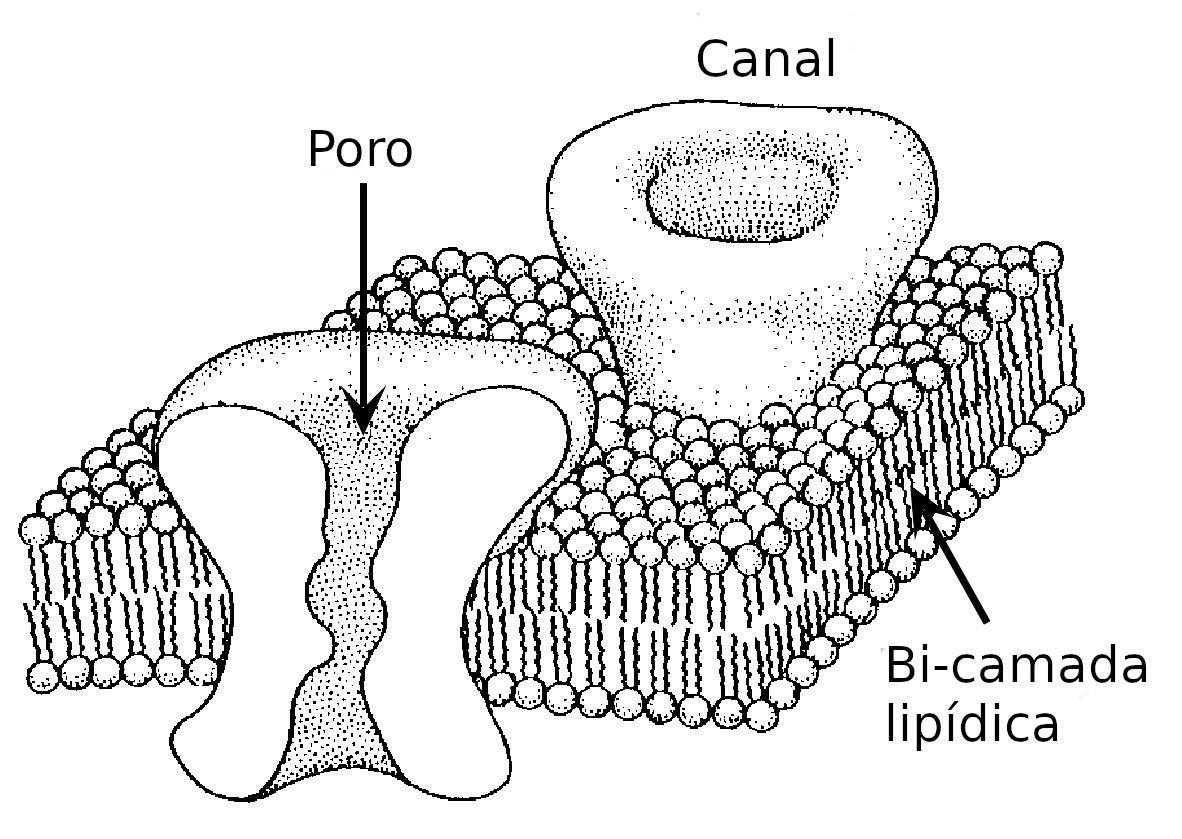
\includegraphics[width=0.55\linewidth]{figs/membrana_neuronio}
				\label{fig:membrananeuronio}
%				\fonte{adaptado de \cite{hille_ionic_1992}}
			\end{figure}
		\column{5cm}
			\begin{itemize}
				\item O interior da célula, geralmente, possui mais cargas negativas;
				\item o potencial de membrana fica a maior parte do tempo negativo;
				\note{potencial de membrana: diferença entre o potencial interno e o externo da célula neuronal}
				\item o fluxo de íons através dos poros de canais iônicos altera o potencial de membrana.
			\end{itemize}
	\end{columns}
\end{frame}

\begin{frame}
	\begin{columns}[t]
		\column{5cm}
			\begin{figure}[tb!]
				\centering
				\caption{Canais iônicos de potássio}
				\label{fig:canaisions}
				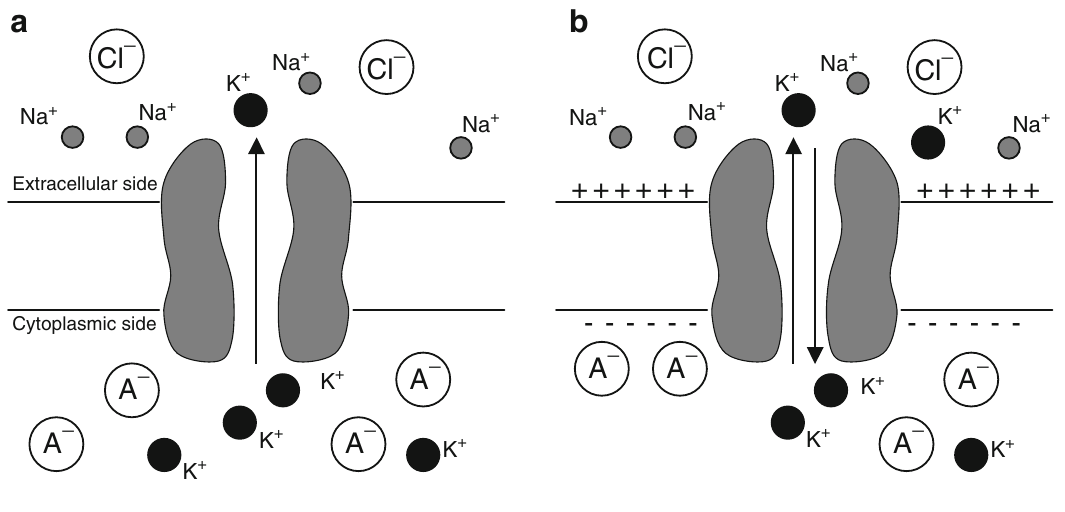
\includegraphics[width=0.7\linewidth]{figs/canais_ions}
%				\fonte{Adaptado de \cite{ermentrout_mathematical_2010}}
			\end{figure}
		\column{5cm}
			\begin{itemize}
				\item Canais iônicos permitem a movimentação de íons através deles;
				\item podem ser sem portão, que estão sempre abertos, ou com portão, que podem abrir ou fechar;
				\item quando não há fluxo de íons e o potencial de membrana não se altera ele é chamado de potencial de repouso.
				\note{valor típico do potencial de repouso: $-70\ mv$}
			\end{itemize}
	\end{columns}
\end{frame}

\begin{frame}
	\begin{columns}[t]
		\column{5cm}
			\begin{itemize}
				\item Despolarização: quando íons positivos entram na célula, deixando o potencial de membrana mais positivo;
				\item Hiperpolarização: quando íons negativos entram na célula, ou positivos saem, deixando o potencial de membrana mais negativo;
				\item o potencial de membrana é dado na forma de uma equação diferencial.
			\end{itemize}
		\column{5cm}
			\[
				\frac{\mathrm{d}V_m}{\mathrm{d}t}=G_l(E_l-V_m)/C_m
			\]
			\begin{itemize}
				\item $V_m$: potencial de membrana
				\item $C_m$: capacitância da membrana
				\item $E_l$: potencial de vazamento
				\item $G_l$: condutância de vazamento
			\end{itemize}
	\end{columns}
\end{frame}

\subsection*{Equações diferenciais ordinárias}
\begin{frame}
	teste
\end{frame}
